\section{方法}
\label{sec:methods}

\subsection{传播与报告模型}
\label{sec:meth-model}

考虑第 $t$ 期的传播（图~\ref{fig:model}）。上一代有 $n$ 名感染者，第 $i$ 人产生 $X_{i,t}$ 个继发感染。为刻画超传播，沿用 Lloyd-Smith 等\citep{lloydsmith2005superspreading}的设定，令给定 $R_t$ 时各 $X_{i,t}$ 相互独立，且服从如下负二项分布：
\begin{equation}
  X_{i,t}\mid R_t \sim \NB(k,\ k/(k+R_t)),\qquad
  \E(X_{i,t}\mid R_t)=R_t,\quad \Var(X_{i,t}\mid R_t)=R_t+\frac{R_t^2}{k}.
  \label{eq:offspring}
\end{equation}
其中 $k$ 为离散参数，$k$ 越小，传播越集中于少数个体。式~\eqref{eq:offspring} 等价于个体再生数服从均值为 $R_t$、形状参数为 $k$ 的 Gamma 分布，继发感染数在其上服从泊松分布\citep{lloydsmith2005superspreading, endo2020estimating}。新感染总数 $I_t=\sum_{i=1}^{n}X_{i,t}$ 中，每人独立地以概率 $\rho$ 被报告，即 $C_t\mid I_t\sim\Bin(I_t,\rho)$。

负二项分布 $\NB(r,p)$ 取“失败次数”参数化时，概率母函数为 $G(s)=p^{r}[1-(1-p)s]^{-r}$。独立和的母函数等于各项之积，所以 $I_t\sim\NB(nk,p)$，$p=k/(k+R_t)$。二项稀疏对应复合 $G_C(s)=G_I(1-\rho+\rho s)$；记 $q=1-(1-p)(1-\rho)$，有：
\begin{equation}
  G_C(s)=\frac{p^{nk}}{[q-(1-p)\rho s]^{nk}}=\frac{(p/q)^{nk}}{\{1-[(1-p)\rho/q]\,s\}^{nk}}.
  \label{eq:thinning}
\end{equation}
由于 $1-p/q=(1-p)\rho/q$，式~\eqref{eq:thinning} 正是 $\NB(nk,p/q)$ 的母函数。代入 $p=k/(k+R_t)$ 得 $p/q=k/(k+\rho R_t)$，报告数的条件分布因此为：
\begin{equation}
  C_t\mid n, R_t \sim \NB(nk,\ k/(k+\rho R_t)),\qquad
  \E(C_t\mid n,R_t)=\rho n R_t,\quad
  \Var(C_t\mid n,R_t)=\rho n R_t+\frac{\rho^2 n R_t^2}{k}.
  \label{eq:report-dist}
\end{equation}
记 $m=\rho n$，即上一代感染者中预计被报告的人数，下文称为预计报告规模，并用它度量监测规模。报告数的相对方差由两部分组成：
\begin{equation}
  \frac{\Var(C_t\mid n,R_t)}{\E(C_t\mid n,R_t)^2}=\frac{1}{\rho n R_t}+\frac{1}{nk}.
  \label{eq:relvar}
\end{equation}
第一项来自报告抽样，提高报告率 $\rho$ 可以压低它；第二项来自超传播，只能靠增加感染者人数 $n$ 压低。

\begin{figure}[!tbp]
  \centering
  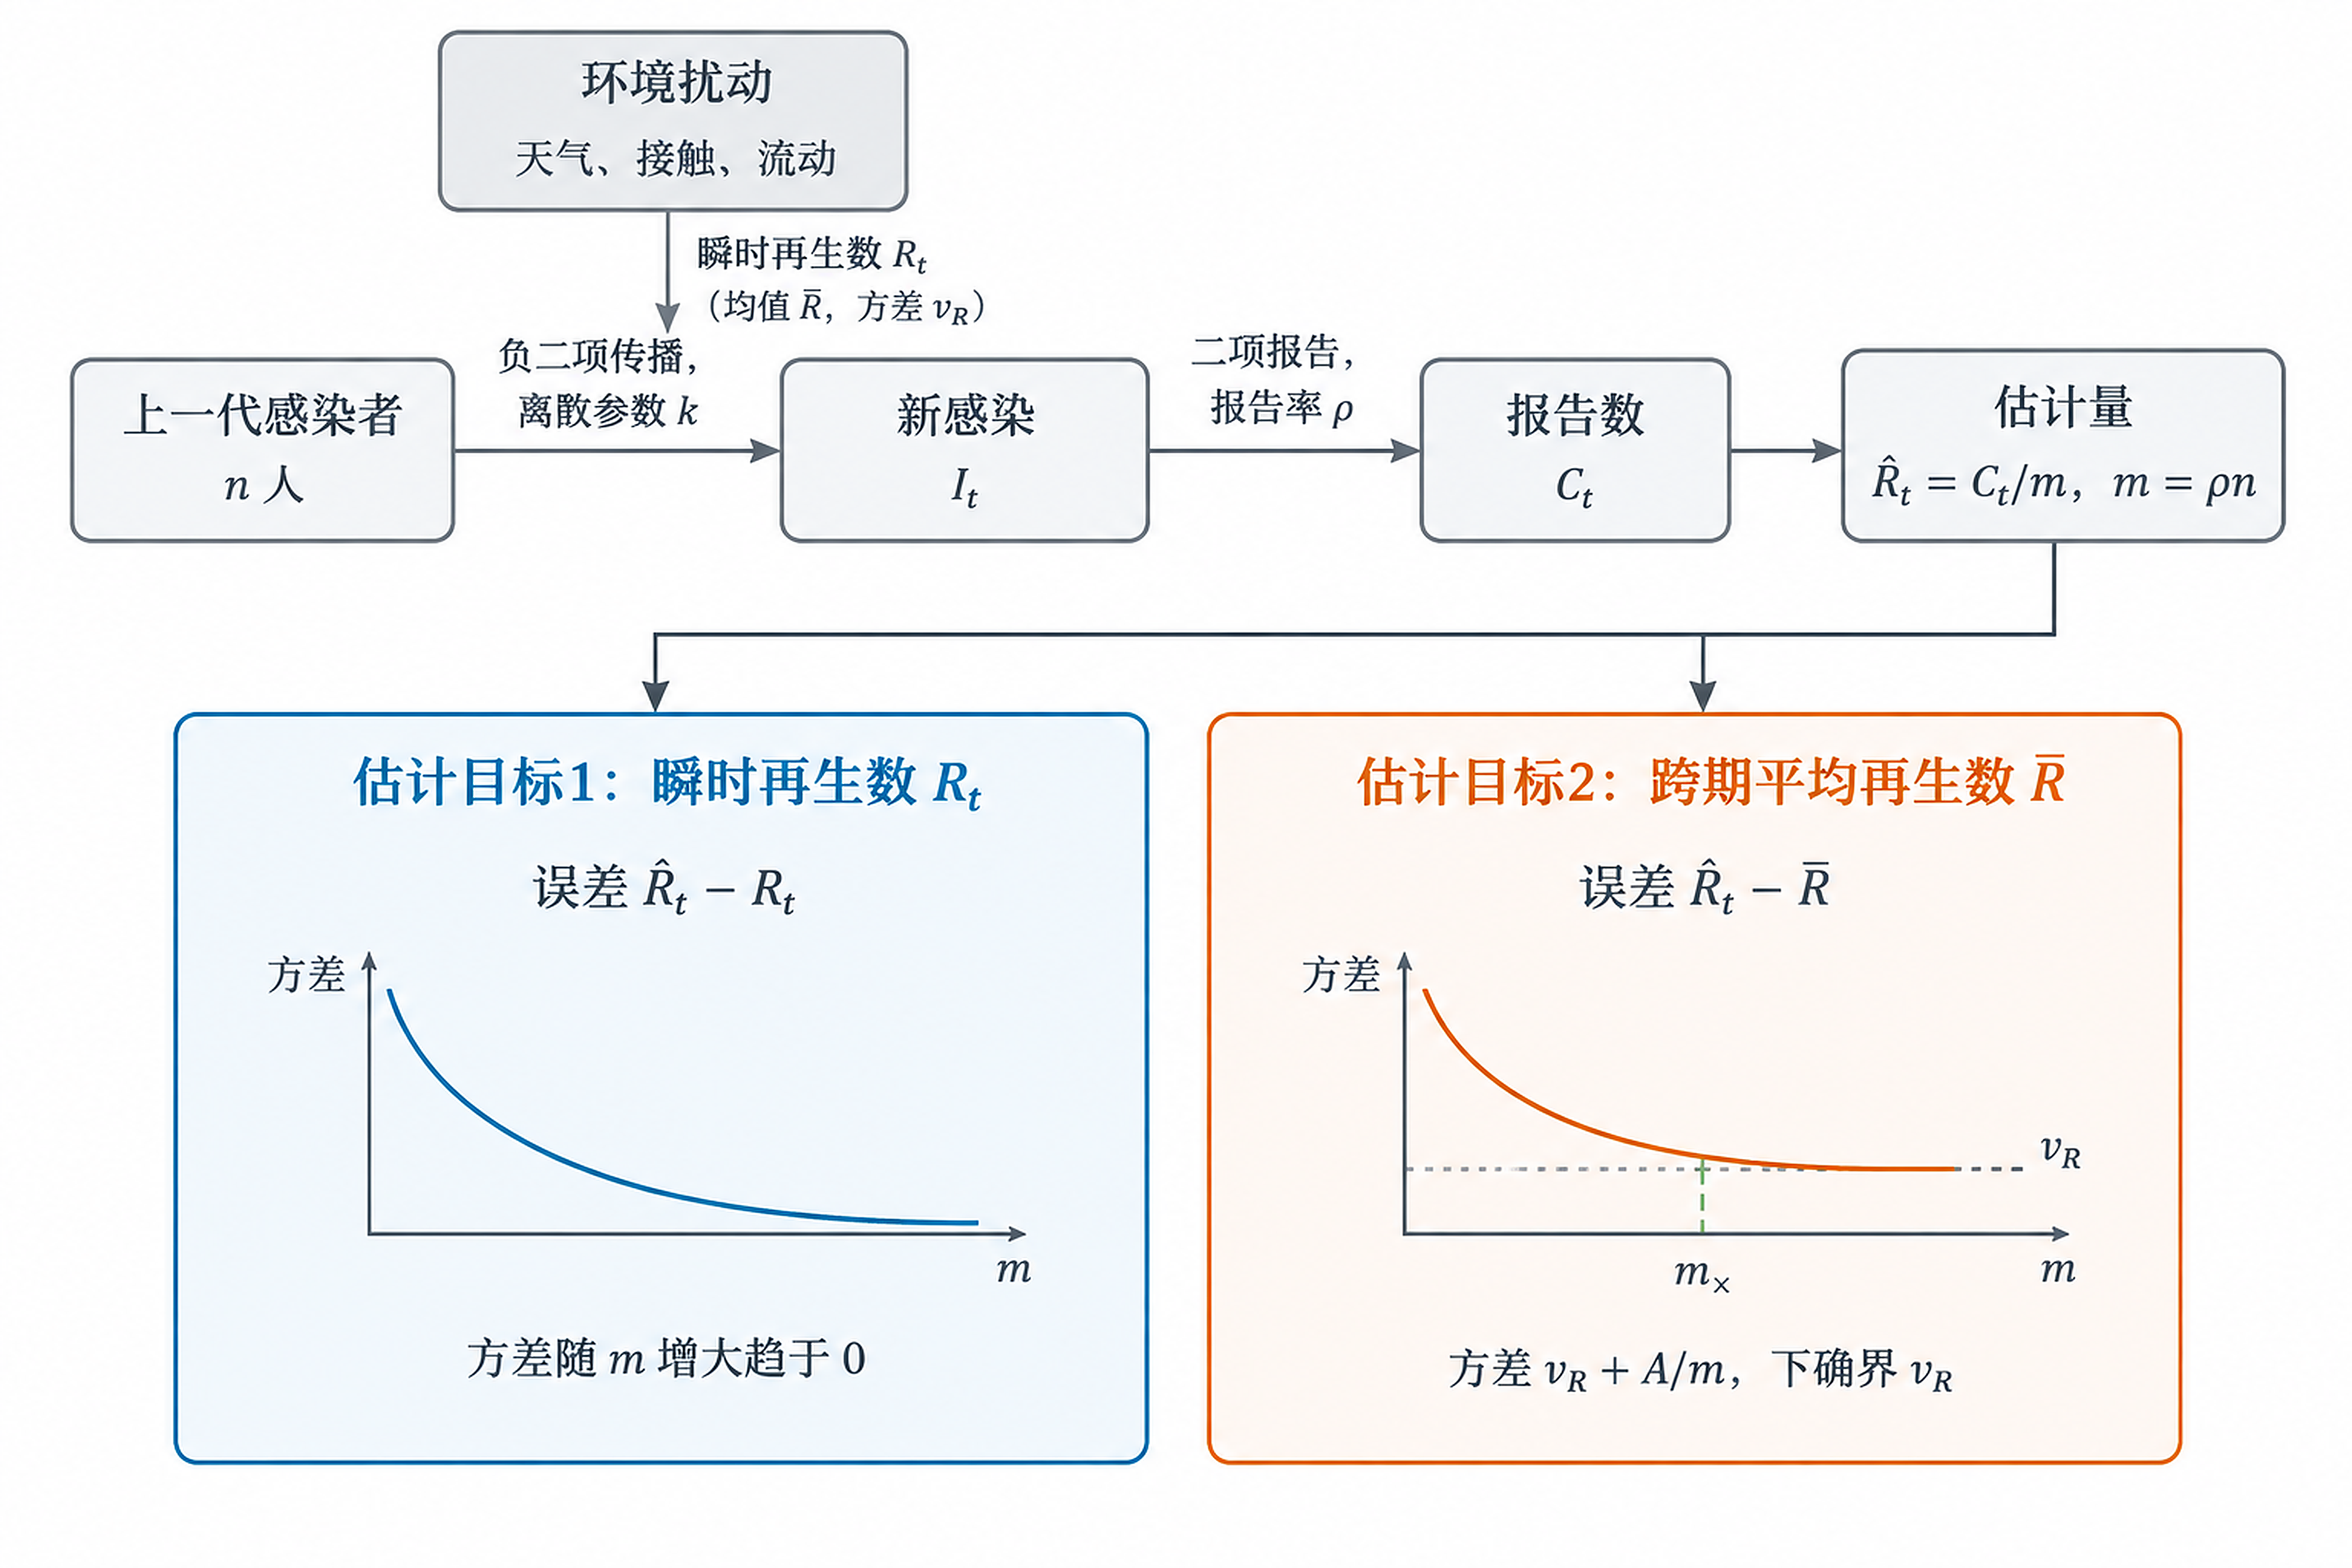
\includegraphics[width=0.92\textwidth]{figures/fig_01_model_schematic.png}
  \caption{模型与两个估计目标的示意。上排为传播与报告过程。环境扰动决定当期瞬时再生数 $R_t$，上一代 $n$ 名感染者按负二项分布产生新感染 $I_t$，新感染经二项报告成为报告数 $C_t$，由此得到估计量 $\widehat R_t=C_t/m$。下排为同一估计量对应的两个估计目标，估计目标1的误差方差随预计报告规模 $m$ 趋于零；估计目标2的误差方差为 $v_R+A/m$，在对 $R_t$ 条件无偏的估计类中以环境方差 $v_R$ 为下确界。下排曲线只示意变化形状，不对应具体参数。}
  \label{fig:model}
\end{figure}

\subsection{两个估计目标与模型假设}
\label{sec:meth-targets}

$R_t$ 随时间波动。天气、学校假期和人群流动使各期的传播强度围绕平均水平变化\citep{dalziel2018urbanization, rasmussen2011inference}，记 $\E(R_t)=\Rbar$，$\Var(R_t)=v_R$，称 $v_R$ 为环境方差。生态学把这类同一期内全体个体共享的波动称为环境随机性，以区别于个体层面的人口随机性\citep{engen1998demographic, rohani2002determinism}。

监测问题据此分为两个估计目标。估计目标1是条件估计目标，即给定当期环境时实际发生的瞬时再生数 $R_t$，例如判断本周传播是否快于上周。世代离散且互不重叠时，$R_t$ 与 Cori 等\citep{cori2013new}由更新方程定义的瞬时再生数一致。估计目标2是边缘估计目标，即各期再生数所围绕的跨期平均再生数 $\Rbar$。各期环境独立（$\phi=0$）时，它也是下一期传播水平的一步前瞻预测；$\Rbar$ 由此前 $T_0$ 期估计时，预测误差再乘以 $1+1/T_0$。环境存在时间相关时，前瞻预测可以利用相关性，误差下界降为 $(1-\phi^2)v_R$，两者不再等价。已知下一期的预计报告规模 $m$ 时，以 $\Rbar$ 预测下一期实现的增长 $C_{t+1}/m$，等价于以 $\Rbar m$ 预测下一期报告数。两个目标共用估计量 $\widehat R_t=C_t/m$，区别在于误差的参照对象。估计目标1的误差为 $\widehat R_t-R_t$，估计目标2的误差为 $\widehat R_t-\Rbar$，后者多出一项不随规模变化的 $R_t-\Rbar$。

第~\ref{sec:res-current}--\ref{sec:res-test}~节的推导依赖以下四条假设，第~\ref{sec:r3-reporting}--\ref{sec:r3-design}~节另用关于报告率的 H5 与 H6。
\begin{enumerate}[label=H\arabic*]
  \item 给定 $R_t$，各感染者的继发感染数相互独立且服从式~\eqref{eq:offspring}，报告过程为独立二项抽样。
  \item 同一期的感染者共享同一个 $R_t$，即环境扰动作用在期的层面。
  \item 离散参数 $k$ 与报告率 $\rho$ 已知。
  \item 规模 $n$ 与当期环境无关，即 $\E(R_t\mid n)=\Rbar$，$\Var(R_t\mid n)=v_R$；作一步预测时，还要求 $R_{t+1}$ 与截至第 $t$ 期的全部信息独立。
\end{enumerate}
若 $n$ 由设计固定，例如每期追踪固定数目的指示病例，H4 自然成立。若 $n_t$ 是此前传播的结果，而 $R_t$ 又有时间相关，较大的 $n_t$ 往往出现在 $R_t$ 偏高的时期，H4 不再自动成立。真实监测序列属于后一种情况，第~\ref{sec:meth-renewal}~节的更新过程设定与第~\ref{sec:meth-sim}~节的一阶自回归仿真专门处理它。H3 在实践中也只是近似，$k$ 需要估计。

\subsection{方差的推导}
\label{sec:meth-derivation}

\subsubsection{估计目标2与条件无偏估计类}

称估计量 $\tilde\theta$ 对 $R_t$ 条件无偏，若 $\E(\tilde\theta\mid R_t)=R_t$。把误差拆为 $\tilde\theta-\Rbar=(\tilde\theta-R_t)+(R_t-\Rbar)$，交叉项的期望为 $\E[(R_t-\Rbar)\,\E(\tilde\theta-R_t\mid R_t)]=0$，于是由全方差公式得：
\begin{equation}
  \E(\tilde\theta-\Rbar)^2=\E\big[\Var(\tilde\theta\mid R_t)\big]+v_R
  \ \geq\ v_R+\E\big[1/\mathcal I(R_t)\big]=v_R+\frac{A}{m},\qquad
  A=\Rbar+\frac{\rho(\Rbar^2+v_R)}{k}.
  \label{eq:unbiased-bound}
\end{equation}
不等号对只用本期报告数的估计量成立，由给定 $R_t$ 时的 Cramér--Rao 不等式得到；$\E[1/\mathcal I(R_t)]=\E[R_t/(\rho n)+R_t^2/(kn)]$，其中 $\E(R_t^2)=\Rbar^2+v_R$，由此得到 $A/m$。式~\eqref{eq:unbiased-bound} 中 $v_R$ 这一部分只依赖条件无偏，估计量使用其他期数据时同样成立。由命题~\ref{prop:current} 的得分函数（补充材料 S1.1 节），$\widehat R_t=C_t/m$ 取到等号，$v_R+A/m$ 是该估计类中的最小均方误差。

\subsubsection{一步前瞻预测}

设 $\mathcal F_t$ 为截至第 $t$ 期的全部信息，下一期规模 $m$ 已知。在 H4 下 $R_{t+1}$ 与 $\mathcal F_t$ 独立，对任何以 $\mathcal F_t$ 为依据的预测量 $\hat y$，下一期实现增长 $y=C_{t+1}/m$ 的预测误差满足：
\begin{equation}
  \E(\hat y-y)^2\ \geq\ \Var(y\mid\mathcal F_t)=v_R+\frac{A}{m},
  \label{eq:predict-bound}
\end{equation}
等号由 $\hat y=\Rbar$ 取到。这一下界对所有预测量成立，不需要无偏性限定，但依赖 H4。实际预测中 $\Rbar$ 未知；用此前 $T_0$ 期相互独立、规模同为 $m$ 的 $\widehat R_t$ 的平均值代替时，预测误差为 $(v_R+A/m)(1+1/T_0)$，多出的部分来自基准本身的估计误差。若 $R_t$ 服从系数为 $\phi$ 的平稳一阶自回归，$\Var(R_{t+1}\mid R_t)=(1-\phi^2)v_R$，借用此前各期的信息最多可把不可约的环境部分降到 $(1-\phi^2)v_R$；$\phi=0.5$ 与 $0.8$ 时分别为 $0.75v_R$ 与 $0.36v_R$。若目标换成 $T$ 期平均，环境项变为 $\Var(T^{-1}\sum_t R_t)$，各期独立时为 $v_R/T$，一阶自回归时为\citep{hamilton1994time}：
\begin{equation}
  \Var\Bigl(\frac1T\sum_{t=1}^{T}R_t\Bigr)=\frac{v_R}{T}\Bigl[1+2\sum_{h=1}^{T-1}\Bigl(1-\frac hT\Bigr)\phi^{h}\Bigr]
  =\frac{v_R}{T}\cdot\frac{1+\phi}{1-\phi}-\frac{2\phi(1-\phi^T)\,v_R}{T^2(1-\phi)^2}.
  \label{eq:ar-sum}
\end{equation}
本文的环境方差下确界只针对单期设定，即只用一期数据估计 $\Rbar$，或在 H4 下预测下一期。多期设定由命题~\ref{prop:allocation} 处理，允许条件偏差的收缩估计见补充材料 S1.11 节。

\subsection{更新过程与增长统计量}
\label{sec:meth-renewal}

真实监测序列中，上一代感染者人数 $n$ 未知。下一周的新感染由此前几周的感染共同产生，感染压力为 $\Lambda_{t+1}=\sum_{s\geq1}w_sI_{t+1-s}$，其中 $w_s$ 为世代间隔分布\citep{fraser2007estimating, cori2013new}。漏报使 $I_1,\dots,I_t$ 无法完全观测，$\Lambda_{t+1}$ 在报告信息下也是随机的。可用的只有报告数的加权和 $D_t=\sum_{s\geq1}w_sC_{t+1-s}$，增长统计量取 $G_t=C_{t+1}/D_t$。令 $m=\rho\,\E(\Lambda_{t+1}\mid\mathcal F_t)$。设给定 $\Lambda_{t+1}$ 与 $R_{t+1}$ 时，$C_{t+1}$ 服从式~\eqref{eq:report-dist} 中以 $\Lambda_{t+1}$ 代替 $n$ 的负二项分布，且在 $\mathcal F_t$ 条件下 $\Lambda_{t+1}$ 与 $R_{t+1}$ 独立。两次使用全方差公式（补充材料 S1.12 节），可得：
\begin{equation}
  \frac{\Var(C_{t+1}\mid\mathcal F_t)}{[\rho\,\E(\Lambda_{t+1}\mid\mathcal F_t)]^2}
  =v_R+\frac{A}{m}+\CV^2(\Lambda_{t+1}\mid\mathcal F_t)\,(\Rbar^2+v_R).
  \label{eq:info-decomp}
\end{equation}
$\Lambda_{t+1}$ 完全已知时，变异系数项为零，式~\eqref{eq:info-decomp} 退化为式~\eqref{eq:predict-bound} 的右端。多出的一项来自感染压力的不确定性，它与规模无关，并随漏报程度和世代间隔的展宽而增大。

实证所用的误差指标有两种等价形式。用 $\Rbar D_t$ 预测 $C_{t+1}$ 的相对误差，与用 $G_t$ 估计 $\Rbar$ 的相对误差恒等，即：
\begin{equation}
  \frac{(C_{t+1}-\Rbar D_t)^2}{(\Rbar D_t)^2}=\frac{(G_t-\Rbar)^2}{\Rbar^2}.
  \label{eq:identity}
\end{equation}
记 $\mu_t=\E(C_{t+1}\mid\mathcal F_t)$，$\varsigma_t^2=\Var(C_{t+1}\mid\mathcal F_t)$。$D_t$ 由 $\mathcal F_t$ 决定，增长统计量的均方误差可以分解为：
\begin{equation}
  \E[(G_t-\Rbar)^2]=\E((\varsigma_t/D_t)^2)+\E[(\mu_t/D_t-\Rbar)^2].
  \label{eq:mse-decomp}
\end{equation}
第二项是条件偏差，非负。$D_t$ 只是 $\rho\Lambda_{t+1}$ 的带噪代理，第一项不必等于 $v_R+A/D_t$，单代公式 $(v_R+A/m)/\Rbar^2$ 在时间序列中因此只作参照曲线，一般情况下不构成下界。

以某一阶段的平均增长比 $\Rbar$ 为基准，第 $t$ 周的损失定义为 $L_t=[(G_t-\Rbar)/\Rbar]^2$。由式~\eqref{eq:identity}，它也是用 $\Rbar D_t$ 预测 $C_{t+1}$ 的相对误差平方，属于常用的相对误差评分\citep{bosse2023scoring}。在单代模型中以 $D_t$ 代替 $m$，损失的条件期望为关于 $1/D_t$ 的仿射形式：
\begin{equation}
  \E(L_t\mid D_t)\approx a+\frac{b}{D_t},\qquad a=\frac{v_R}{\Rbar^2},\quad b=\frac{A}{\Rbar^2},\quad \frac ba=\mx.
  \label{eq:affine}
\end{equation}
下文以式~\eqref{eq:affine} 为拟合形式，称 $b/a$ 为经验比值。

分母本身是带二项报告噪声的计数，比真实感染压力 $\rho\Lambda_{t+1}$ 多一层随机性。令 $D_t=m(1+\delta)$，给定真实感染史时 $\E\delta=0$，$\E\delta^2=(1-\rho)\sum_s{w_s}^2/m$。把 $G_t=(C_{t+1}/m)(1+\delta)^{-1}$ 按 delta 方法\citep{casella2002statistical}展开到 $\delta^2$，再以条件均值的平方归一化（补充材料 S1.12 节），斜率近似为：
\begin{equation}
  b\approx\frac{A+(1-\rho)(\Rbar^2+v_R)\sum_s {w_s}^2}{\Rbar^2}.
  \label{eq:b-delta}
\end{equation}
权重越集中，$D_t$ 越接近单周计数，噪声越大，$b$ 也越大。分母或自变量含噪时的系数偏移在测量误差文献中有系统处理\citep{fuller1987measurement, carroll2006measurement}。

式~\eqref{eq:b-delta} 给出三种滞后权重之间斜率之比 $r_j=b_j/b_{\text{主}}$ 的预测；截距之比记为 $q_j=a_j/a_{\text{主}}$。为检验这些比值的判别力，对照了四种机制。M-env 为本文模型，即平稳环境方差加二项分母噪声，截距与权重无关（$q=1$）。M-bin0 取 $v_R=0$，只保留二项分母噪声。M-meas 为纯测量误差模型，误差全部来自分母与分子的报告抽样，均值形状为 $b/D$，没有底板。M-nodn 令分母不含计数噪声，两个斜率比都等于 1。M-mult 为乘性报告噪声，即各周报告比例在州内有共同的随机冲击，截距与命题~\ref{prop:report-noise}(vii) 的 $F(w,\psi)$ 成正比，$\psi$ 为冲击的周间自相关；$\psi=0$ 时 $F=1+\sum_s{w_s}^2$。各机制的预测比值统一按情景 $\Rbar=1.67$ 计算。

\subsection{仿真设计}
\label{sec:meth-sim}

\subsubsection{单代核对}

命题~\ref{prop:current} 与命题~\ref{prop:average} 的蒙特卡洛核对在 $m\in[1,1000]$ 的 10 个规模上各做 20,000 次模拟，随机种子为 20261013，参数为 $\Rbar=1.15$、$v_R=0.04$、$k=0.35$、$\rho=0.25$。增长检验的实际水平与功效全部由负二项分布函数精确计算（式~\eqref{eq:power}），没有模拟误差。

\subsubsection{更新过程}

世代间隔取 4 周离散核，权重依次为 0.45、0.35、0.15、0.05。每周 $R_t$ 独立抽自均值 1.15、方差 0.04 的 Gamma 分布，新感染 $I_t\sim\NB(k\Lambda_t,\,k/(k+R_t))$，$k=0.35$，报告数 $C_t\sim\Bin(I_t,0.25)$。为避免轨迹灭绝，$I_t$ 截断为不小于 1；截断只在小规模时发生，$m_0=6$ 与 12 时的比例分别为 1.42\% 与 0.16\%，$m_0\geq25$ 时为零。前 4 周的感染数设为 $m_0/\rho$，使初始每周预计报告 $m_0$ 例，$m_0$ 从 6 到 800 共取 8 档。每档模拟 400 条 30 周的轨迹，每条轨迹有 26 个评价点，随机种子为 20261014。误差按初始规模 $m_0$ 汇总，或按实现规模 $D_t$ 分组汇总，再与单代参照曲线相除。

\subsubsection{时间相关环境}

为检验 $R_t$ 的时间相关能否解释实证截距的水平，令 $R_t=\max(0.05,\mu_R+e_t)$，$e_t$ 为方差 $v_R$、系数 $\phi$ 的平稳一阶自回归，$\phi=1$ 表示整季恒定偏差。每周一代，感染数服从均值 $R_tI_t$、$k=0.35$ 的负二项分布，报告服从 $\Bin(I_t,0.021)$。共 153 条州--季序列，每条 3 周前置、10 周观测、1 周前瞻；起始规模从实证 153 个州--季的流行初期首周 $D_t$ 中抽取。网格为 $\phi\in\{0,0.3,0.5,0.7,0.9,1\}$、$v_R\in\{0.04,0.08,0.16\}$，以及三组均值与起始规模 $(\mu_R,\text{规模倍数})=(1.67,1)$、$(1.42,1)$ 与 $(1.42,0.25)$。第二组使模拟的平均增长比接近实证的 1.67，第三组再把 $D_t$ 的中位数压到接近实证的 53。每格重复 400 次，随机种子为 20261022。估计口径与实证完全相同。

\subsection{流感住院数据}
\label{sec:meth-data}

数据来自 NHSN 公布的各辖区每周实验室确诊流感住院数，以及各辖区填报医院所占比例\citep{cdc2026nhsn}，样本截至 2026 年 9 月。样本覆盖 50 个州与华盛顿特区，共 16,218 个州周，其中 504 个州周的住院数缺失并按 0 处理，468 个在第一期，36 个在第二期。规模用此前三周报告数的加权和度量：
\begin{equation}
  D_t=0.65\,C_t+0.25\,C_{t-1}+0.10\,C_{t-2}.
  \label{eq:dt}
\end{equation}
相对待预测的 $C_{t+1}$，$D_t$ 的平均回溯滞后为 1.45 周，约 10.2 天。只保留 $D_t\geq5$ 的州周，得到 10,303 个有效观测。敏感性分析另用只用当周和三周等权两种权重。前者的 $\sum w^2=1$，平均滞后 1.0 周；后者的 $\sum w^2=0.333$，平均滞后 2.0 周。主规格的 $\sum w^2=0.495$。

样本期内 NHSN 的填报制度变过两次。2020 年 10 月至 2024 年 4 月 30 日为强制填报（第一期），有效观测 6,009 个，平均填报率 91.1\%。2024 年 5 月 1 日至 10 月 31 日改为自愿填报（第二期），有效观测 420 个，平均填报率 54.6\%，中位数 45.7\%。2024 年 11 月 1 日起，美国联邦医疗保险与医疗补助服务中心恢复强制要求（第三期），有效观测 3,874 个，平均填报率 91.8\%。流行季定义为 10 月至次年 3 月。

流行初期窗口为 2022 年 10 月 8 日至 11 月 26 日、2023 年 10 月 14 日至 12 月 16 日、2024 年 11 月 9 日至 2025 年 1 月 18 日。达峰期窗口为三个流行季的全国峰值周（2022 年 12 月 3 日、2023 年 12 月 30 日、2025 年 2 月 8 日）及其后 7 周。

\subsection{统计推断}
\label{sec:meth-inference}

式~\eqref{eq:affine} 用可行广义最小二乘拟合，权重取 $1/\hat\mu^2$，$\hat\mu$ 为上一轮的拟合值，迭代至系数收敛\citep{wooldridge2010econometric}。只迭代一步时主规格系数几乎不变（$a=0.0991$，$b=2.242$），单周规格的斜率由 3.134 变为 3.102。区间由按州聚类的 2,000 次重抽给出。每次有放回地抽 51 个州，三种权重共用同一组抽样，每次重抽都重估基准 $\Rbar$ 并重新拟合\citep{cameron2008bootstrap, cameron2015practitioner}。正文报告 95\% 百分位区间；偏差校正加速（BCa）区间\citep{efron1987better}的加速度由留一州刀切估计，与百分位区间的差别远小于区间宽度。敏感性分析另按州 $\times$ 流行季（153 簇）聚类，以及按周聚类。

均值形状的比较在主规格流行初期样本上进行，预先设定了三个模型，即 $L=b/D$（无底板）、$L=a+b/D$ 与 $L=cD^{-p}$（无底板的幂律）。各模型用方差与均值平方成正比的 Gamma 准似然拟合\citep{mccullagh1989generalized}，它与上述加权方式一致。比较的指标为 AIC 与留一州交叉验证的 Gamma 偏差，留一州时 $\Rbar$ 只用训练州估计，报告逐州差值之和及州间标准误。判定规则在运行比较之前写定。

填报制度期之间的离散度用 $G_t$ 的四分位距比较，另用连续性校正的对数增长率 $\log[(C_{t+1}+0.5)/(D_t+0.5)]$ 的四分位距去掉增长水平对离散度的伸缩作用。区间来自按州聚类的 2,000 次重抽，各格与差值在同一次抽样内计算。季节构成用三种方式控制。第一种按全面板的季内占比 0.580 重新加权；第二种为同月份对照，即第二期的 5--9 月和 10 月分别与其他年份同月比较；第三种为分位数回归\citep{koenker1978regression}。分位数回归的因变量为对数增长率与当月全样本中位数之差的绝对值，协变量为期别、流行季与 $\log D_t$，扩展模型再加入期别 $\times$ 流行季交互。中位数与 0.75 分位数回归的区间分别来自 500 次与 250 次州聚类重抽。敏感性分析剔除 $t-2$ 至 $t+1$ 任一周住院数缺失的 12 个州周。

工具变量回归以滞后 3--5 周的规模作 $1/D_t$ 的工具，区间由 10,000 次重抽给出。事前基准有三种口径，即全部历史扩张窗、26 周滚动池和逐州扩张窗，均只使用预测时点以前的数据。Cori 等\citep{cori2013new}的滑动窗口基准取 1、2、3 周窗，窗口内感染压力之和不足 5 例的州周不参与比较。外部数据中，FluSight 集成预测与欧洲 COVID-19 序列分别取自文献\citep{mathis2024evaluation, flaxman2020estimating}公开的数据，聚类单位分别为州和国家。

\subsection{报告率、规模与期数及跨病原复制的分析}
\label{sec:meth-r3}

本节的分析在运行前写定了判据，运行后追加的分析在正文中标为事后分析。区间来自按州聚类的 2,000 次重抽（随机种子 20261017）。流感流行初期的主分析报告百分位区间，跨病原比较与报告调整报告 BCa 区间。第~\ref{sec:r3-reporting}--\ref{sec:r3-design}~节的蒙特卡洛核对使用同一种子。

报告率代理取 NHSN 公布的各州每周填报医院比例，记为 $\hat p_{s,t}$；用填报医院数作代理的敏感性分析给出相同结果。由命题~\ref{prop:report-noise}(vi)，州内恒定的报告率在 $G_t$ 中约去，进入截距的是比值 $\pi_{s,t}=\hat p_{s,t+1}/\sum_jw_j\hat p_{s,t-j}$ 的方差 $V_\pi$。报告调整估计量把各周计数换成 $C^*_{s,t}=C_{s,t}/\hat p_{s,t}$，按同样的滞后权重得到 $D^*_t$ 与 $G^*_t=G_t/\pi_{s,t}$，行集合与未调整版本相同，再按第~\ref{sec:meth-inference}~节的方式对 $1/D_t$ 拟合式~\eqref{eq:affine}，得到 $a^*$ 与截距比 $q_1^*$、$q_2^*$；敏感性分析改对 $1/D^*_t$ 回归。$\Delta a=a-a^*$ 与两组截距共用同一组重抽。判据写定如下。$\Delta a$ 的下端大于 0 且点估计不低于 0.02 时，认为可观测的报告成分对截距有可检出的贡献；否则以 $\Delta a$ 区间的上端作为这一贡献的上界。运行前还写下了两支预测：若 $\hat p$ 正是计数的报告因子，$\Delta a\approx+V_\pi(1+a)$；若填报比例的周间变化与计数无关，调整只增加噪声，$\Delta a\approx-V_\pi(1+a)$。另有两项分析同样在运行前写定。一是等价检验，以 $a$ 的 5\% 为等价界，$\Delta a$ 的 90\% BCa 区间落在界内时，认为可观测报告成分的贡献与 0 等价。二是报告率网格仿真（35 格，每格 200 次，种子 20261060），检验 $\Delta a$ 判据在已知报告波动下的水平与功效。

规模与期数的比较对应命题~\ref{prop:vR-info}。降规模不降期数的做法是对每个州的周计数做二项稀疏 $C'\sim\Bin(C,p)$，$p\in\{0.5,0.25\}$，每次重抽重新稀疏；降期数不降规模的做法是每次只抽一半或四分之一的州。判据针对州平均 $D_t$ 高于中位数的 25 个大州，要求 $p=0.5$ 的稀疏使 $a$ 的区间宽度增加不超过 15\%，而州数减半使宽度增加至少 30\%。另报告三个流行季各自的截距、季间异质性的 $Q$ 检验与留一季估计。事后分析把季作为随机效应，用 DerSimonian--Laird 估计季间方差\citep{dersimonian1986meta}，区间取自由度为 $S-1$ 的 $t$ 分位数。

跨病原复制使用同一 NHSN 文件中的 COVID-19 与 RSV 住院数及各自的填报医院比例。窗口有两种，一种与流感相同的日历窗口（RSV 只有 2024--2025 季有强制填报数据），另一种为增长期窗口，即全国合计增长比 $G^{\mathrm{nat}}_t\geq1.05$ 的周，从 2022 年 8 月起，剔除第二期，RSV 从 2024 年 11 月起。同一规则用于流感，其 2025--2026 季的增长期不在主分析样本中，作为样本外季。各病原的截距超出按自身的 $\Rbar$ 计算为 $a-0.08/\Rbar^2$，0.08 是流感情景中 $v_R$ 的上端。判据如下。零假设范围由两组增长期仿真给出，按各病原组合的世代间隔与增长率设定，每格模拟 300 次。一组为环境各期独立（$\phi=0$）的日分辨率更新过程，取环境变异系数平方 CV$^2$（周再生数的方差与均值平方之比）4 档、世代间隔 3 档、入院延迟 3 档（无、短、长）与增长率 3 档，共 108 格（种子 20261058）。另一组为 $v_R=0$ 的增长期乘性报告噪声模型，报告冲击服从对数一阶自回归，取 $\psi\in\{0,0.3,0.6,0.9\}$、$\tau\in\{0.15,0.3\}$、入院延迟 2 档与增长率 3 档，共 48 格（种子 20261059）。零假设范围取两组格点模拟平均的最小值至最大值之并。$q_1$ 与 $q_2$ 的 95\% BCa 区间都与该范围不相交，且截距超出量区间的下端大于 0，称为复现。两项只满足其一，称为部分复现；两项都不满足、但两个区间仍在 $q_1<1<q_2$ 的方向上排除 1，称为方向一致。判断区间是否与零假设参数集合相交即置信区间反演检验，零假设范围因此不再用模拟分位数加宽。方向一致只作辅助描述，不称为复现。
